\documentclass{article}

\textwidth=6.5in
\textheight=8.5in
\voffset=-54pt
\oddsidemargin=0in
\evensidemargin=0in
\setlength{\parskip}{8pt}
\setlength{\parindent}{0pt}

\usepackage{amsmath, amssymb}
\usepackage{ifthen}

\usepackage[inline]{enumitem}
\setlist{topsep=0pt, parsep=8pt}

\usepackage[rgb,table]{xcolor}\convertcolorsUfalse
\usepackage{graphicx}

% change hyperref options
\PassOptionsToPackage{hyphens}{url}
\usepackage[bookmarks,colorlinks,linkcolor=black,citecolor=blue,pdfstartview=FitH,urlcolor=blue]{hyperref}
\hypersetup{pdfpagemode=UseNone}
\usepackage{bookmark}

\usepackage{graphicx}
\usepackage{multicol}
\usepackage{framed}
\usepackage{array}

\usepackage{icomma}

\usepackage{soul}
\usepackage[normalem]{ulem}

\usepackage{pgfplots}
\pgfplotsset{compat=1.18}  
\pgfplotscreateplotcyclelist{mycolor}{black, blue, red, green!70!black, magenta, purple, cyan, orange }  
\pgfplotsset{
  disabledatascaling,
  cycle list=tikzcolor, 
  axis lines=middle,
  every axis plot/.style={no marks, thick},
  every axis/.style={
    enlarge x limits=false,
    enlarge y limits=auto,
    xlabel style={at={(current axis.right of origin)},anchor=west},
    ylabel style={at={(current axis.above origin)},anchor=south},
    % extra x and y ticks for asymptotes
    extra x tick style={grid=major, grid style={dashed,black}},
    extra y tick style={grid=major, grid style={dashed,black}},
    /pgf/number format/1000 sep={},
  },    
  tick label style = {font=\footnotesize, fill=\currentbgcolor, inner sep=0pt},    
  xticklabel shift=1pt,    
  scaled ticks=false,
  scaled y ticks=false,
  unbounded coords=jump,
  samples=101,
  minor tick length=0,
  scatter/classes={
    open={mark=*,draw=black,fill=white, mark size=2, thin},
    closed={mark=*,draw=black,fill=black, mark size=2, thin}
  },
  width=3in,
}
\pgfplotsset{open/.style={only marks, mark=*, fill=white, thin, mark size=2}}
\pgfplotsset{closed/.style={only marks, mark=*, draw=black, fill=black,
    thin, mark size=2}}
\pgfplotsset{labeled/.style={nodes near coords, only marks, mark=*, draw=black, fill=black, thin, mark size=2, point meta=explicit symbolic}}

\usepackage{tikz}
\usetikzlibrary{
  matrix,%
  % enables the snake paths
  decorations.pathmorphing,%
  % enables bigger arrows
  decorations.markings,%
  decorations.pathreplacing,%
  decorations.text,%
  calc,%
  patterns,%
  shapes.geometric,%
  arrows,
  decorations.shapes,
  positioning,
  plotmarks,
  intersections
}
\tikzset{>=latex} % sets default arrow type in tikz
\tikzset{font=\normalsize}
\tikzset{mark size=1.5pt, mark options=thin}
\tikzset{pin distance=4pt,
  every pin edge/.style={<-, thin, shorten <= -2pt}}

\interfootnotelinepenalty=10000
\renewcommand{\thefootnote}{(\arabic{footnote})}

\usepackage{multirow, bigdelim}

% change to \usepackage[sols]{handout} to see solutions
\usepackage[]{handout}

\newcommand\iscurrentenumi[1]{%
  \ifthenelse{\equal{#1}{\theenumi}}{}{#1}}
\setenumerate[1]{ref=\#\arabic*}
\setenumerate[2]{ref=\protect\iscurrentenumi{\theenumi}(\alph*)}
\newcommand\enumiiprefix[2]{%
  \ifthenelse{{\equal{#1}{\theenumi}}\AND{\equal{#2}{(\alph{enumii})}}}{}{}%
  \ifthenelse{{\equal{#1}{\theenumi}}\AND{\NOT{\equal{#2}{(\alph{enumii})}}}}{#2}{}%
  \ifthenelse{\equal{#1}{\theenumi}}{}{#1#2}%
}
\setenumerate[3]{ref=\protect\enumiiprefix{\theenumi}{(\alph{enumii})}\roman*}

\newlength{\tipmargin}
\makeatletter

\newdimen\SOUL@dimen %new
\def\SOUL@ulunderline#1{{%
    \setbox\z@\hbox{#1}%
    % \dimen@=\wd\z@
    \SOUL@dimen=\wd\z@ %new
    \dimen@i=\SOUL@uloverlap
    \advance\SOUL@dimen2\dimen@i %\dimen@ exchanged too
    \rlap{%
      \null
      \kern-\dimen@i
      % \SOUL@ulcolor{\SOUL@ulleaders\hskip\dimen@}%
      \SOUL@ulcolor{\SOUL@ulleaders\hskip\SOUL@dimen}% new
    }%
    \unhcopy\z@
  }}

\renewenvironment{framed}{
  \setlength{\tipmargin}{\textwidth-\linewidth}
  \advance\@totalleftmargin-\tipmargin
  \def\FrameCommand{\hspace{\tipmargin}\fbox}%
  \advance\linewidth\tipmargin
  \MakeFramed {\advance\hsize-\width \FrameRestore}%
}
{\endMakeFramed}

\makeatother

\definecolor{purple}{rgb}{0.5,0,1.0}

\usepackage{fancyhdr}
\lhead{\textcolor{white}{This content is protected and may not be shared, uploaded, or distributed.}}
\rhead{}
\rfoot{\vspace*{\fill}\footnotesize\textcopyright{} \emph{Harvard Math Ma}}
\renewcommand{\headrulewidth}{0pt}
\pagestyle{fancy}
\begin{document}

\htitle{22. Introduction to Exponential Functions}

\begin{problemonly}
  \begin{framed}

You should be able to:
    \begin{itemize}[topsep=0pt,partopsep=0pt,parsep=8pt,itemsep=0pt]
    \item Model quantities that have a constant percent change (per unit of input). 

    \item Graph $b^x$ for different values of $b$ (and be able to combine this with what we know about altering functions to graph functions involving $b^x$).

    \item Apply exponent rules. 
    \end{itemize}
  \end{framed}
\end{problemonly}

\begin{enumerate}
\item 

  \note{We will often want to contrast linear functions and exponential functions, so this problem reminds students a bit about linear functions. I won't give students too long to work on this since this isn't really the emphasis.}

  \emph{Investment scenario 1}. On his birthday last year, Lin invested \$1,000 in a small company. A year later, he discovers that his investment has grown in value by \$100 so is now worth \$1,100. Suppose that Lin's investment grows at a constant rate.

  \begin{enumerate}
  \item
    \begin{problem}
      Fill in the table below.

      { \renewcommand{\arraystretch}{1.5}
        \begin{tabular} {l | l}
          $t$ & Value of Lin's investment after $t$ years \\  \hline
          0& \$1000  \\ 
          1& \\ 
          2 & \\ 
          3 & \\ 
        \end{tabular}
      }
    \end{problem}

    \begin{solution}
      \begin{center}
        \begin{tabular} {c | c}
          $t$ & Value of investment after $t$ years \\  \hline
          0&\$1000  \\
          1& \$1000 + \$100 = \$1100\\ 
          2 & \$1100 +\$100 = \$1200 \\ 
          3 & \$1200 + \$100 = \$1300 \\ 
        \end{tabular}
      \end{center} 
    \end{solution}

  \item

    \note{This probably won't come up, but students may question whether it makes sense to model this as a continuous function. If your bank only credits you with interest once a year, then the account value should be more like a step function. This is a totally reasonable interpretation, but we've seen already that we often model discrete situations using continuous models.

      If students don't ask, I won't bring this up. }

    \begin{problem}[\stretch{0.5}]
      Write a function giving the value of Lin's investment after $t$
      years.  What type of function is this?
    \end{problem}

    \begin{solution} The modeling assumption in this
      problem is that the rate of change is constant and is equal to
      $100 \frac{\$}{\text{year}}$. \textcolor{blue}{A constant rate
        of change is the defining quality of a linear function}, so we
      know that $f(x)$ is going to be a linear function. The slope of
      the function is $100$ and the $y-$intercept is $1000$
      $$f(x) = 100x+1000$$ 
    \end{solution}

  \item

    \note{The key point I want students to see is that, although the rate of change of Lin's investment with respect to time is constant, the annual percent change decreases.}

    \begin{problem}[\vfill\newpage]
      By what percent does the value of Lin's investment increase in the first year? The second year? The third?
    \end{problem}

    \begin{solution}
      To calculate percent change we use the following formula:
      $$ \text{\% change} = \frac{\text{new value} - \text{initial value} }{\text{initial value}}$$ 
      During the first year:
      $$ \frac{ f(1) - f(0) }{f(0)}=\frac{100}{1000} = 10\%$$ 
      During the second year:
      $$ \frac{ f(2) - f(1) }{f(1)}=\frac{100}{1100} \approx 9 \%$$ 
      During the third year:
      $$ \frac{ f(3) - f(2) }{f(2)}=\frac{100}{1200} \approx 8.3 \%$$ 
      We can see that the percent change is decreasing; this makes sense because the account grows by \$100 each year, but the account value keeps growing, so that \$100 represents a smaller and smaller percent of the account value.
    \end{solution}

  \end{enumerate}

\item  \emph{Investment scenario 2.} Lex also invested \$1,000 last year, but suppose that her investment grows by 10\% each year.
  \begin{enumerate}
  \item

    \note{We saw that Lin's account grows by 10\% in the first year but by less than 10\% in each subsequent year, so we can tell Lex is better off even without calculating the value of Lex's investment each year.}

    \begin{problem}[0.75in]
      Is Lin or Lex better off in the long run?  How do you know?
    \end{problem}

    \begin{solution}
      In the first year, Lin's account and Lex's account grow by the same percent. But every year after that, Lex's account grows by a greater percent, so Lex's account will have more money after the first year.
    \end{solution}

  \item

    \begin{problem}[\vfill]
      Fill in the table below. Do you see a pattern? (Hint: If something increases by 10\%, it gets multiplied by \fitb{0.5in}{1.1}.)

      \renewcommand{\arraystretch}{1.5}
      \begin{tabular} {c | l}
        $t$ & Value of Lex's investment after $t$ years \\  \hline
        0& \$1000  \\ 
        1& \\ 
        2 & \\ 
        3 & 
      \end{tabular}
    \end{problem}

    \begin{solution}
      Since ``increases by 10\%'' is the same as ``gets multiplied by 1.1'', we have
      \begin{center}
        \begin{tabular} {c | l}
          $t$ & Value of Lex's investment after $t$ years \\  \hline
          0& \$1000  \\ 
          1& $\$1000 (1.1)$ \\ 
          2 &$\$1000 (1.1) (1.1) = \$1000 (1.1)^2$ \\ 
          3 & $\$1000 (1.1)^2 (1.1) = \$1000 (1.1)^3$ 
        \end{tabular}
      \end{center}
    \end{solution}

  \item

    \begin{problem}[\vfill]
      Write a function giving the value of Lex's investment after $t$ years.
    \end{problem}

    \begin{solution}
      $g(t) = 1000 (1.1)^t$
    \end{solution}

  \end{enumerate}

\end{enumerate}
\begin{framed}
  \smallskip
  An exponential function is a function of the form $f(x) =
  \fitb{2.5in}{C \cdot b^x \text{ where } b > 0}$.
  \begin{itemize}
  \item If money is changing \uline{\emph{linearly}} over time, that means it changes by the same \fitb{1.25in}{amount} each year.

  \item If money is changing \uline{\emph{exponentially}} over time, that means it changes by the same \fitb{1.25in}{percent} each year.

    Another way of saying the same thing is that the amount of money is \solonly{\textbf{multiplied by the same factor each year}.}

    \probonly{\bigskip}
  \end{itemize}
\end{framed}

\pspace{\newpage}

\begin{enumerate}[resume]
\item \label{milk}

  \note{Students may want to say $20 (0.02)^t$ or $20(1.02)^t$ or $20(-0.02)^t$, so be prepared to help them understand why these aren't right.}

  \begin{problem}
    In a certain town in 1975, the amount of whole milk consumed by the average resident was 20 gallons (over the entire year). Since 1975, that consumption has been decreasing by $2\%$ each year. 
\end{problem}
    \begin{enumerate}
    \item (Fill in the blank.) The yearly percent change is (choose one: $\pm$)\fitb{.25in}{-} \fitb{1.25in}{2}\%.

    \item Given this yearly percent change, what percent remains after each year?
    \begin{solution}
        98\%
    \end{solution}

\begin{problemonly}
    \vfill
\end{problemonly}

    \item In order to calculate the percent of milk consumption you found in part (b), what decimal should you multiply by?
\begin{problemonly}
    \vfill
\end{problemonly}
    \begin{solution}
        0.98
    \end{solution}
    
    \item Write a formula for $M(t)$, the amount of whole milk consumed by the average resident $t$ years after 1975.
  
\begin{problemonly}
    \vfill
\end{problemonly}
  \begin{solution} 
     $M(t) = 20 \cdot 0.98^t$
  \end{solution}
\end{enumerate}

\item  \note{ Help students pay careful attention to when $2^x$ is above $3^x$.

    When we discuss this, I would also like to talk about how $2^x$ and $\left( \frac{1}{2} \right)^x$ relate. I hope students will realize that they look like reflections of each other over the $y$-axis, and we'll talk about why this makes sense. }

  \begin{problem}[\stretch{0.5}]
    On the following set of axes, graph $y = 2^x$, $y = 3^x$, and
    $y = \left( \frac{1}{2} \right)^x$.  Label all intercepts and
    asymptotes.  (Also indicate which graph is which.)

    \begin{tikzpicture}
      \begin{axis}[xmin=-1, xmax=1, ymin=-1, ymax=1, xtick=\empty, 
        ytick=\empty, width=4in, height=4in] 

      \end{axis}
    \end{tikzpicture}
  \end{problem}  

  \begin{solution}
    \tikzset{mylabel/.style  args={at #1 #2  with #3}{
        postaction={decorate, 
          decoration={
            markings, 
            mark= at position #1
            with  \node [#2] {#3};
          } } } }
    \begin{center} 

      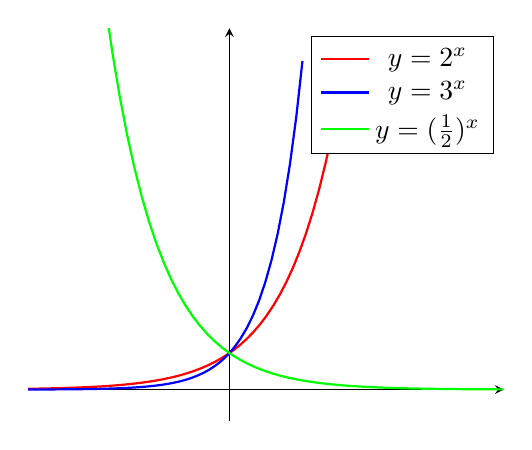
\begin{tikzpicture}[scale=1]
        \begin{axis}[xmin=-3, xmax=5, cycle list={ thick}, axis
          equal=true, ticks=none] 
          \addplot+[domain=-15:3] [red] {2^x};
          \addplot+[domain=-15:2] [blue] {3^x};	
          \addplot+[domain=-10:10] [green] {.5^x};
          \legend{$y=2^x$, $y=3^x$, $y=(\frac{1}{2})^x$}
        \end{axis}
      \end{tikzpicture}
    \end{center} 
    What are the commonalities between the three graphs? 
    All three graphs have one intercept at $(0, 1)$, and a horizontal asymptote at $y=0$.      
    Make sure that you can explain why $3^0 = 1$, or why $3^{-1} = \frac{1}{3}$.
    \textcolor{blue}{You will remember these rules of exponents better by understanding
    why they make sense, not by trying to memorize a long list of rules.} If you're not
    sure why they make sense, work on Question \ref{rules} and see if you can
    see how it would apply to $3^0=1$ and $3^{-1}=\frac{1}{3}$.

    Q: What do you notice when we look at the graphs for  $y=(\frac{1}{2})^x$ and $y=2^x$? Can you explain this observation? \\ A: $y=2^x$ is a reflection of $y=(\frac{1}{2})^x$ about the $y$-axis. This makes sense, because we can rewrite $y=(\frac{1}{2})^x$ as $y=2^{-x}$.

    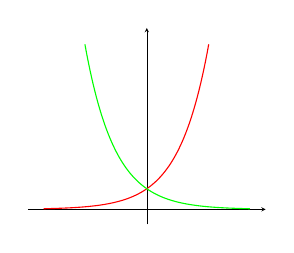
\begin{tikzpicture}[scale=.5]
      \begin{axis}[xmin=-4, xmax=4, cycle list={ thick}, axis
        equal=true, ticks=none] 
        \addplot+[domain=-5:3] [red] {2^x};
        \addplot+[domain=-3:5] [green] {.5^x};
      \end{axis}
      \end{tikzpicture}
  \end{solution}

\item Formalizing the existence of asymptotes, evaluate the following limits: \\
For values of $b>1$
$$\lim_{x\to \infty} b^x = \fitb{0.5in}{\infty}\,\,  \lim_{x\to -\infty} b^x = \fitb{0.5in}{0}$$\\
For values of $b$ between 0 and 1, ($0<b<1$)
$$\lim_{x\to \infty} b^x = \fitb{0.5in}{0}\,\,  \lim_{x\to -\infty} b^x = \fitb{0.5in}{\infty}$$\\


\end{enumerate}
\begin{framed}
  We call $f(x) = C \cdot b^x$ an \uline{exponential growth function} if $C > 0$ and $b \fitb{0.5in}{> 1}$, and we call it an \uline{exponential decay function} if $C > 0$ and $b \fitb{0.5in}{< 1}$. 
\end{framed}

\begin{enumerate}[resume, topsep=0pt]
\item 

  \note{Make sure students recognize that we don't know the derivative of $2^x$, but we can still answer this because we can see the graph of $2^x$ is increasing and concave up everywhere. Some students will probably want to try to apply the Power Rule to say that the derivative of $2^x$ is $x \cdot 2^{x - 1}$. (I will probably try to convince them this is wrong by observing that this is negative when $x < 0$, which isn't consistent with the graph of $2^x$.)}

  \begin{problem}[\nstretch{1}]
    If $f(x) = 2^x$, what can you say about the signs of $f'(x)$ and
    $f''(x)$?
  \end{problem}

  \begin{solution}
    Since the function is increasing everywhere, $f'(x)>0$ everywhere.
    Since the function is concave up everywhere, $f''(x) >0$
    everywhere.
  \end{solution}

\item 

  \begin{problem}[\stretch{2.5}]
    Sketch the graph of $3 \left( \frac{4}{3} \right)^x - 5$, and label the $y$-intercept and any asymptotes. Is this the same as $4^x - 5$?
  \end{problem}

  \begin{solution}
    We know that the $y$-intercept is $3(\frac{4}{3})^0-5=-2$. As $x\to\infty$,
    the function grows without bound. As $x\to-\infty$, $(\frac{4}{3})^x$ approaches
    zero, so there is a horizontal asymptote at $y=-5$.
    \begin{tikzpicture}
      \begin{axis}[ymin=-10, extra y ticks={-5}, ytick={-2}]
        \addplot+[domain=-7:7] {3*(4/3)^x-5};
      \end{axis}
    \end{tikzpicture}
    
    This is not the same as $y=4^x-5$, which would have a $y$-intercept at $y=-1$ and
    would grow much faster than $y=3(\frac{4}{3})^x -5$.
  \end{solution}

\item  \label{rules}

  \note{Students have done something like this way back in \href{https://people.math.harvard.edu/~jjchen/mathma/docs/workshops/workshop01.html}{Workshop 1}, {{\#1}}. Remind them that we can figure out these rules by thinking of $b^x$ as multiplying $x$ copies of $b$.}

  Your friend is having a hard time remembering how exponents work. Help them figure out how to rewrite each of the expressions below, and explain why those rules make sense.
  \begin{multicols}{3}
    \begin{enumerate}
    \item $b^x b^y = \solonly{\bm{b^{x + y}}}$
    \item $\left( b^x \right)^y = \solonly{\bm{b^{xy}}}$
    \item $(ab)^x = \solonly{\bm{a^x b^x}}$
    \end{enumerate}
  \end{multicols}

  \pspace{\vfill}

  \begin{solution} 
    We can convince ourselves that the rules identified
      above our correct by using examples.
      \begin{enumerate}
      \item[(b)] Below we use both an equation and words to describe an
        example. Understanding the example helps us see why the general
        rule is true.
        \begin{center} $\textcolor{blue}{6}^{\textcolor{brown}{3}} \cdot\textcolor{blue}{6}^{\textcolor{green!70!black}{5}} = \textcolor{purple}{(\textcolor{blue}{6} \cdot \textcolor{blue}{6} \cdot \textcolor{blue}{6})}\textcolor{green!70!black}{ (\textcolor{blue}{6}\cdot \textcolor{blue}{6} \cdot \textcolor{blue}{6} \cdot \textcolor{blue}{6} \cdot \textcolor{blue}{6}) }= \textcolor{blue}{6}^{\textcolor{brown}{3}+\textcolor{green!70!black}{5}} =\textcolor{blue}{6}^8$. \\
          If I multiply \textcolor{purple}{three} \textcolor{blue}{sixes}
          with \textcolor{green!70!black}{five} \textcolor{blue}{sixes}, I
          will end up with \textcolor{purple}{three} plus
          \textcolor{green!70!black}{five} \textcolor{blue}{sixes} or
          eight \textcolor{blue}{sixes}. \end{center}
      \item[(c)] Can you come up with an example for this one?
        \begin{center}
          $(\textcolor{blue}{5}^{\textcolor{brown}{2}}
          )^{\textcolor{green!70!black}{3}} =
          \textcolor{green!70!black}{(\textcolor{blue}{5}^{\textcolor{brown}{2}}
            \cdot \textcolor{blue}{5}^{\textcolor{brown}{2}} \cdot
            \textcolor{blue}{5}^{\textcolor{brown}{2}} )}=
          \textcolor{blue}{5}^{\textcolor{brown}{2}\cdot
            \textcolor{green!70!black}{3}} =\textcolor{blue}{5}^6$.
        \end{center}
        A critical observation in the above example is that \begin{center}
          $\textcolor{green!70!black}{(\textcolor{blue}{5}^{\textcolor{brown}{2}}
            \cdot \textcolor{blue}{5}^{\textcolor{brown}{2}} \cdot
            \textcolor{blue}{5}^{\textcolor{brown}{2}} )}=
          \textcolor{blue}{5}^{\textcolor{brown}{2}\cdot
            \textcolor{green!70!black}{3}}$
        \end{center}
        This follows since there are \textcolor{green}{3} groups of
        \textcolor{brown}{2} \textcolor{blue}{fives}.
      \end{enumerate} 
  \end{solution}

\item 
  Simplify the following expression as much as possible. (You should be able to write them all so there are no fractions left.)

  \begin{enumerate}

  \item
    \begin{problem}[\vfill]
      $\dfrac{(ab^2)^x}{b^x}$
    \end{problem}

    \begin{solution}
      \begin{align*}
        \frac{(ab^2)^x}{b^x} &= \frac{a^xb^{2x}}{b^x} \\
        &= a^x \frac{b^{2x}}{b^x} \\
        &= a^x b^{(2x-x)} \\
        &= \boxed{a^x b^x}
      \end{align*}
    \end{solution}

  \item

    \note{This is to give us a chance to talk about the fact that there isn't a rule for $b^x + b^y$}

    \begin{problem}[\vfill]
      $\dfrac{b^{2x} + b^{3x}}{b^x}$
    \end{problem}

    \begin{solution}
      \begin{align*}
        \frac{b^{2x}+b^{3x}}{b^x} &= \frac{b^{2x}}{b^x} + \frac{b^{3x}}{b^x} \\
        &= \boxed{b^x + b^{2x}}
      \end{align*}
    \end{solution}

  \item
    \begin{problem}[\nstretch{1.5}]
      $\displaystyle \frac{C \cdot 4^{t + 1} - C \cdot 4^t}{C \cdot 4^{t}}$
    \end{problem}

    \begin{solution}
      \begin{align*}
        \frac{C \cdot 4^{t + 1} - C \cdot 4^t}{C \cdot 4^t} &= \frac{C \cdot
          4^t ( 4 - 1)}{C \cdot 4^t} \\
        &= 4 - 1 \\
        &= \boxed{3}
      \end{align*}
    \end{solution}

  \item
    \begin{problem}[\vfill]
      $\dfrac{(3a)^{2x} - \left( a^2 \right)^x}{\sqrt{a^x a^{3x}}}$ where $a > 0$
    \end{problem}

    \begin{align*}
       \frac{(3a)^{2x} - \left( a^2 \right)^x}{\sqrt{a^x a^{3x}}} &=
       \frac{3^{2x}a^{2x} - a^{2x}}{(a^{4x})^{1/2}} \\
       &= \frac{a^{2x}(3^{2x}-1)}{a^{2x}} \\
       &= \boxed{3^{2x} -1}
    \end{align*}

  \item

    \begin{problem}[\vfill]
      $\displaystyle \frac{2^{3x} + \sqrt{9 \cdot 6^{4x}}}{4^x}$ 
    \end{problem}

    \begin{solution}
      \begin{align*}
        \frac{2^{3x} + \sqrt{9 \cdot 6^{4x}}}{4^x} &= \frac{2^{3x} +
          \sqrt{9} \sqrt{6^{4x}}}{4^x} \\
        &= \frac{2^{3x} + 3 \sqrt{6^{4x}}}{4^x} \\
        &= \frac{2^{3x}}{4^x} + 3 \frac{\sqrt{6^{4x}}}{4^x} \\
        &= \frac{8^x}{4^x} + 3 \frac{6^{2x}}{4^x} \\
        &= \left( \frac{8}{4} \right)^x + 3 \frac{ (6^2)^x}{4^x} \\
        &= 2^x + 3 \left( \frac{6^2}{4} \right)^x \\
        &= \boxed{2^x + 3 \cdot 9^x}
      \end{align*}
    \end{solution}

  \end{enumerate}

\item \label{bacteria}

  A scientist is growing some bacteria in a petri dish. Suppose the petri dish starts with 100 bacteria, and the number of bacteria doubles each hour. Let $B(t)$ be the number of bacteria in the petri dish after $t$ hours.
  \begin{enumerate}
  \item
    \begin{problem}[1in]
      Write a formula for $B(t)$. 
    \end{problem}

    \begin{solution}
        $B(t) = 100 \cdot 2^t$.
    \end{solution}

  \item

    \note{The fact that doubling is an $100\%$ increase can be confusing to students. (This is also in the Edfinity, so don't feel like you need to do this problem.)}

    \begin{problem}[1in]
      What is the percent change per hour in the number of bacteria? 
    \end{problem}

    \begin{solution}
      Each hour the amount of bacteria is multiplied by $2$. This is a $100\%$ increase.
    \end{solution}

  \item

    \note{We will do problems like this next time, so again don't feel like you need to do this. I've just put it here in case some students move really quickly through the algebra.}

    \begin{problem}[\vfill\newpage]
      Write a formula for the number of bacteria in the petri dish after $d$ \uline{days}. (Hint: if we know the bacteria multiplies by a given factor each hour, consider how many times we'd like to multiply by that factor each day.)
    \end{problem}

    \begin{solution}
      If $t$ is the number of hours since the start, then $d=\frac{1}{24}t$,
      which means $t=24d$. Since $B=100\cdot 2^t$, we can
      substitute $t=24d$ to get $B = 100\cdot 2^{24d}$.
    \end{solution}

  \end{enumerate}

\item 
  Sketch graphs of the following functions, and label all intercepts and asymptotes.

  \begin{enumerate}
  \item
    \begin{problem}[\vfill]
      $f(x) = -1.5 (0.6)^x$
    \end{problem}

    \begin{solution}
    The $y$-intercept is $(0, -1.5)$ and the horizontal asymptote is $y=0$. No $x$-intercepts.
    
      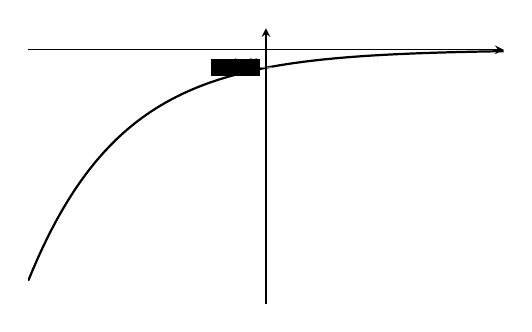
\begin{tikzpicture}
        \begin{axis}[set layers, axis on top, ytick={-1.5},height=2in, xtick=\empty]
          \addplot[domain=-5:5]{-1.5*(0.6)^x};
        \end{axis}
      \end{tikzpicture}
    \end{solution}

  \item
    \begin{problem}[\vfill]
      $g(t) = 10 + 1.5^t$
    \end{problem}

    \begin{solution}
    The $y$-intercept is $(0, 11)$ and the horizontal asymptote is $y=10$. No $x$-intercepts.
    
      \begin{tikzpicture}
        \begin{axis}[set layers, axis on top, ytick={11}, extra y ticks={10}, xtick=\empty]
          \addplot[domain=-5:5]{10+(1.5)^x};
          \addplot[draw=none] {0};
        \end{axis}
      \end{tikzpicture}
    \end{solution}

  \item
    \begin{problem}[\vfill]
      $j(x) = 2 - 4^{-x}$
    \end{problem}

    \begin{solution}
    The $y$-intercept is $(0, 1)$ and the horizontal asymptote is $y=2$. There
    is an $x$-intercept.
    \begin{align*}
     2-4^{-x} &= 0 \\
     2 &= 4^{-x} \\
     \intertext{We can rewrite the left-hand side to have
     the same base as the right-hand side.}
     4^{1/2} &= 4^{-x} \\
     \intertext{Now we can set the exponents equal to each other.}
     \tfrac{1}{2} &= -x \\
     -\tfrac{1}{2} &= x
    \end{align*}
    
      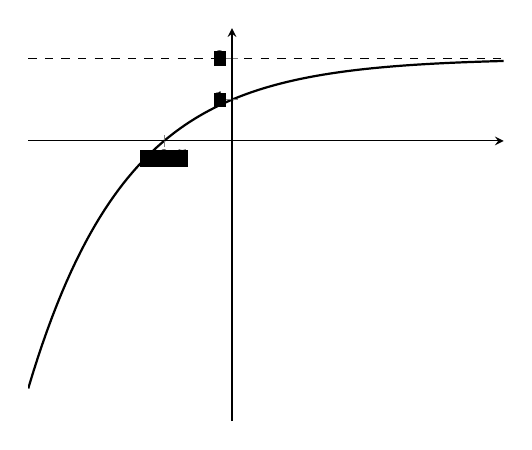
\begin{tikzpicture}
        \begin{axis}[set layers, axis on top, ytick={1}, extra y ticks={2}, xtick={-0.5}]
          \addplot[domain=-1.5:2]{2-4^(-x)};
        \end{axis}
      \end{tikzpicture}
    \end{solution}

  \end{enumerate}
\end{enumerate}
\end{document}
